%!TeX encoding = UTF-8
%!TeX program = xelatex
\documentclass[notheorems, aspectratio=54]{beamer}
% aspectratio: 1610, 149, 54, 43(default), 32

\usepackage{latexsym}
\usepackage{amsmath,amssymb}
\usepackage{mathtools}
\usepackage{color,xcolor}
\usepackage{graphicx}
\usepackage{subfigure}
\usepackage{algorithm}
\usepackage{amsthm}
\usepackage{lmodern} % 解决 font warning
% \usepackage[UTF8]{ctex}
\usepackage{animate} % insert gif

\usepackage{lipsum} % To generate test text 
\usepackage{ulem} % 下划线,波浪线

\usepackage{listings} % display code on slides; don't forget [fragile] option after \begin{frame}

% ----------------------------------------------
% tikx
\usepackage{framed}
\usepackage{tikz}
\usepackage{pgf}
\usepackage{diagbox}
\usetikzlibrary{calc,trees,positioning,arrows,fit,chains,shapes.geometric,%
    decorations.pathreplacing,decorations.pathmorphing,shapes,%
    matrix,shapes.symbols}
\pgfmathsetseed{1} % To have predictable results
% Define a background layer, in which the parchment shape is drawn
\pgfdeclarelayer{background}
\pgfsetlayers{background,main}

\definecolor{AmethystPurple}{HTML}{AEAEDF}
\definecolor{MyRed}{HTML}{FF5959}
% define styles for the normal border and the torn border
\tikzset{
  normal border/.style={AmethystPurple, decorate, 
     decoration={random steps, segment length=2.5cm, amplitude=.7mm}},
  torn border/.style={AmethystPurple, decorate, 
     decoration={random steps, segment length=.5cm, amplitude=1.7mm}}}

% Macro to draw the shape behind the text, when it fits completly in the
% page
\def\parchmentframe#1{
\tikz{
  \node[inner sep=1.5em] (A) {#1};  % Draw the text of the node
  \begin{pgfonlayer}{background}  % Draw the shape behind
  \fill[normal border] 
        (A.south east) -- (A.south west) -- 
        (A.north west) -- (A.north east) -- cycle;
  \end{pgfonlayer}}}

% Macro to draw the shape, when the text will continue in next page
\def\parchmentframetop#1{
\tikz{
  \node[inner sep=2em] (A) {#1};    % Draw the text of the node
  \begin{pgfonlayer}{background}    
  \fill[normal border]              % Draw the ``complete shape'' behind
        (A.south east) -- (A.south west) -- 
        (A.north west) -- (A.north east) -- cycle;
  \fill[torn border]                % Add the torn lower border
        ($(A.south east)-(0,.2)$) -- ($(A.south west)-(0,.2)$) -- 
        ($(A.south west)+(0,.2)$) -- ($(A.south east)+(0,.2)$) -- cycle;
  \end{pgfonlayer}}}

% Macro to draw the shape, when the text continues from previous page
\def\parchmentframebottom#1{
\tikz{
  \node[inner sep=2em] (A) {#1};   % Draw the text of the node
  \begin{pgfonlayer}{background}   
  \fill[normal border]             % Draw the ``complete shape'' behind
        (A.south east) -- (A.south west) -- 
        (A.north west) -- (A.north east) -- cycle;
  \fill[torn border]               % Add the torn upper border
        ($(A.north east)-(0,.2)$) -- ($(A.north west)-(0,.2)$) -- 
        ($(A.north west)+(0,.2)$) -- ($(A.north east)+(0,.2)$) -- cycle;
  \end{pgfonlayer}}}

% Macro to draw the shape, when both the text continues from previous page
% and it will continue in next page
\def\parchmentframemiddle#1{
\tikz{
  \node[inner sep=2em] (A) {#1};   % Draw the text of the node
  \begin{pgfonlayer}{background}   
  \fill[normal border]             % Draw the ``complete shape'' behind
        (A.south east) -- (A.south west) -- 
        (A.north west) -- (A.north east) -- cycle;
  \fill[torn border]               % Add the torn lower border
        ($(A.south east)-(0,.2)$) -- ($(A.south west)-(0,.2)$) -- 
        ($(A.south west)+(0,.2)$) -- ($(A.south east)+(0,.2)$) -- cycle;
  \fill[torn border]               % Add the torn upper border
        ($(A.north east)-(0,.2)$) -- ($(A.north west)-(0,.2)$) -- 
        ($(A.north west)+(0,.2)$) -- ($(A.north east)+(0,.2)$) -- cycle;
  \end{pgfonlayer}}}

% Define the environment which puts the frame
% In this case, the environment also accepts an argument with an optional
% title (which defaults to ``Example'', which is typeset in a box overlaid
% on the top border
\newenvironment{parchment}[1][Example]{%
  \def\FrameCommand{\parchmentframe}%
  \def\FirstFrameCommand{\parchmentframetop}%
  \def\LastFrameCommand{\parchmentframebottom}%
  \def\MidFrameCommand{\parchmentframemiddle}%
  \vskip\baselineskip
  \MakeFramed {\FrameRestore}
  \noindent\tikz\node[inner sep=1ex, draw=black!20,fill=AmethystPurple, 
          anchor=west, overlay] at (0em, 1em) {\sffamily#1};\par}%
{\endMakeFramed}

% ----------------------------------------------

\mode<presentation>{ 
    \usetheme{Warsaw}
    % Boadilla CambridgeUS
    % default Antibes Berlin Copenhagen
    % Madrid Montpelier Ilmenau Malmoe
    % Berkeley Singapore Warsaw
    \usecolortheme{dolphin}
    % beetle, beaver, orchid, whale, dolphin
    \useoutertheme{infolines}
    % infolines miniframes shadow sidebar smoothbars smoothtree split tree
    \useinnertheme{circles}
    % circles, rectanges, rounded, inmargin
}
% 设置 block 颜色
\setbeamercolor{block title}{bg=AmethystPurple,fg=white}

\newcommand{\reditem}[1]{\setbeamercolor{item}{fg=red}\item #1}

% 缩放公式大小
\newcommand*{\Scale}[2][4]{\scalebox{#1}{\ensuremath{#2}}}

% 解决 font warning
\renewcommand\textbullet{\ensuremath{\bullet}}

% ---------------------------------------------------------------------
% flow chart
\tikzset{
    >=stealth',
    punktchain/.style={
        rectangle, 
        rounded corners, 
        % fill=black!10,
        draw=white, very thick,
        text width=6em,
        minimum height=2em, 
        text centered, 
        on chain
    },
    largepunktchain/.style={
        rectangle,
        rounded corners,
        draw=white, very thick,
        text width=10em,
        minimum height=2em,
        on chain
    },
    line/.style={draw, thick, <-},
    element/.style={
        tape,
        top color=white,
        bottom color=blue!50!black!60!,
        minimum width=6em,
        draw=blue!40!black!90, very thick,
        text width=6em, 
        minimum height=2em, 
        text centered, 
        on chain
    },
    every join/.style={->, thick,shorten >=1pt},
    decoration={brace},
    tuborg/.style={decorate},
    tubnode/.style={midway, right=2pt},
    font={\fontsize{10pt}{12}\selectfont},
}
% ---------------------------------------------------------------------

% code setting
\lstset{
    language=C++,
    basicstyle=\ttfamily\footnotesize,
    keywordstyle=\color{red},
    breaklines=true,
    xleftmargin=2em,
    numbers=left,
    numberstyle=\color[RGB]{222,155,81},
    frame=leftline,
    tabsize=4,
    breakatwhitespace=false,
    showspaces=false,               
    showstringspaces=false,
    showtabs=false,
    morekeywords={Str, Num, List},
}

% ---------------------------------------------------------------------

%% preamble
\title{On Dependency Analysis of NPM}
\subtitle{Data Collection \& Case Study}
\author{Cui Zihan}
\institute[ICS NJU]{I2EC, ICS, NJU}

% -------------------------------------------------------------

\begin{document}

%% title frame
\begin{frame}
    \titlepage
\end{frame}

\begin{frame}
    \frametitle{Sections}
    \tableofcontents
\end{frame}

%% normal frame
\section{Review}
\begin{frame}
    \frametitle{Sections}
    \tableofcontents[currentsection]
\end{frame}

\begin{frame}
    \frametitle{Vulnerability Propagation Problem}
    \tikzset{
        normalCircle/.style = {
            draw,
            circle,
            node distance=1.5cm,
            minimum size=0.7cm,
            fill=none
        }
    }

    \center
    \begin{tikzpicture}
        \node[normalCircle, fill=MyRed,] (f0) {$f_0$};
        \node[normalCircle, right of=f0, yshift=0.75cm] (f1) {$f_1$};
        \node[normalCircle, fill=MyRed,below of=f1] (f2) {$f_2$};
        \node[normalCircle, right of=f1, yshift=0.75cm] (f3) {$f_3$};
        \node[normalCircle, fill=MyRed,below of=f3] (f4) {$f_4$};
        \node[normalCircle, right of=f2, yshift=-0.75cm] (f5) {$f_5$};
        \node[normalCircle, fill=MyRed,below of=f5] (f6) {$f_6$};
        \node[normalCircle, fill=MyRed,right of=f4] (f7) {$f_7$};
        \node[normalCircle, fill=MyRed,right of=f5] (f8) {$f_8$};
        \draw[<-, >=latex] (f0) -- (f1);
        \draw[<-, >=latex] (f0) -- (f2);
        \draw[<-, >=latex] (f1) -- (f3);
        \draw[<-, >=latex] (f2) -- (f5);
        \draw[<-, >=latex] (f2) -- (f6);
        \draw[<-, >=latex] (f4) -- (f7);
        \draw[AmethystPurple] (0.75,2)--(0.75,-3.5);
        \draw[AmethystPurple] (2.25,2)--(2.25,-3.5);
        \draw[AmethystPurple] (3.75,2)--(3.75,-3.5);
        \node at (0,2.2) {$P_0$};
        \node at (1.5,2.2) {$P_1$};
        \node at (3,2.2) {$P_2$};
        \node at (4.5,2.2) {$P_3$};
    \end{tikzpicture}

    \begin{figure}
        \caption{Graphical description of a vulnerability propagation problem. }
    \end{figure}
\end{frame}

\begin{frame}
    \frametitle{Review Problem Formulation}
    \begin{block}{Problem Formulation}
        Suppose we have $G = <V,E>$ and $V=\bigcup_{i=0}^{m} P_i$. Where $P_0$ denotes the entry package of the analysed project. Denote $D=\{f_{k1}, f_{k2}\cdots f_{kn}\}$ where $f_{ki}$ refers to a vulnerable function.

        Find if "$\exists f_i \in P_0, f_j \in D, f_i\ is\ reachable\ from\ f_j.$ "holds.
    \end{block}
\end{frame}

\begin{frame}
    \frametitle{Review Research Questions}
    \begin{block}{RQ 1}
        How to judge if $<f_i, f_j>$ exists?
    \end{block}
    \begin{exampleblock}{RQ 2}
        How to tell if $f_i \in D$?
        \begin{itemize}
            \item Resolve functions  and construct the function call graph from packages;
            \item Judge if a function is vulnerable; To solve this problem, we must collect data related to the vulnerabilities. 
        \end{itemize}
    \end{exampleblock}
    \begin{block}{RQ 3}
        How to construct the function call graph within reasonable time?
    \end{block}
\end{frame}

\section{Data Collection}
\begin{frame}
    \tableofcontents[currentsection]
\end{frame}

\begin{frame}
    \frametitle{Data Source}
    We researched the databases of vulnerability records in NPM ecosystem. We find 3 relatively comprehensive data sources, and they have their own advantages and disadvantages:
    \begin{itemize}
        \item CVE(Common Vulnerabilities and Exposures): Supervised by MITRE Corporation; Highly recognized; Lack of a detailed description of the vulnerability; Open source;  
        \item Snyk.io: Provide the most detailed description; Maintained by Snyk, one of the leading companies involved in analysing software vulnerabilities; Commercial;
        \item \textcolor{MyRed}{NPM security advisory}: Maintained by NPM; Open source;
    \end{itemize}
\end{frame}

\begin{frame}
    \frametitle{Data Source}
    \begin{figure}[htbp]
        \centering
        \subfigure{
        \begin{minipage}[t]{0.3\linewidth}
        \centering
        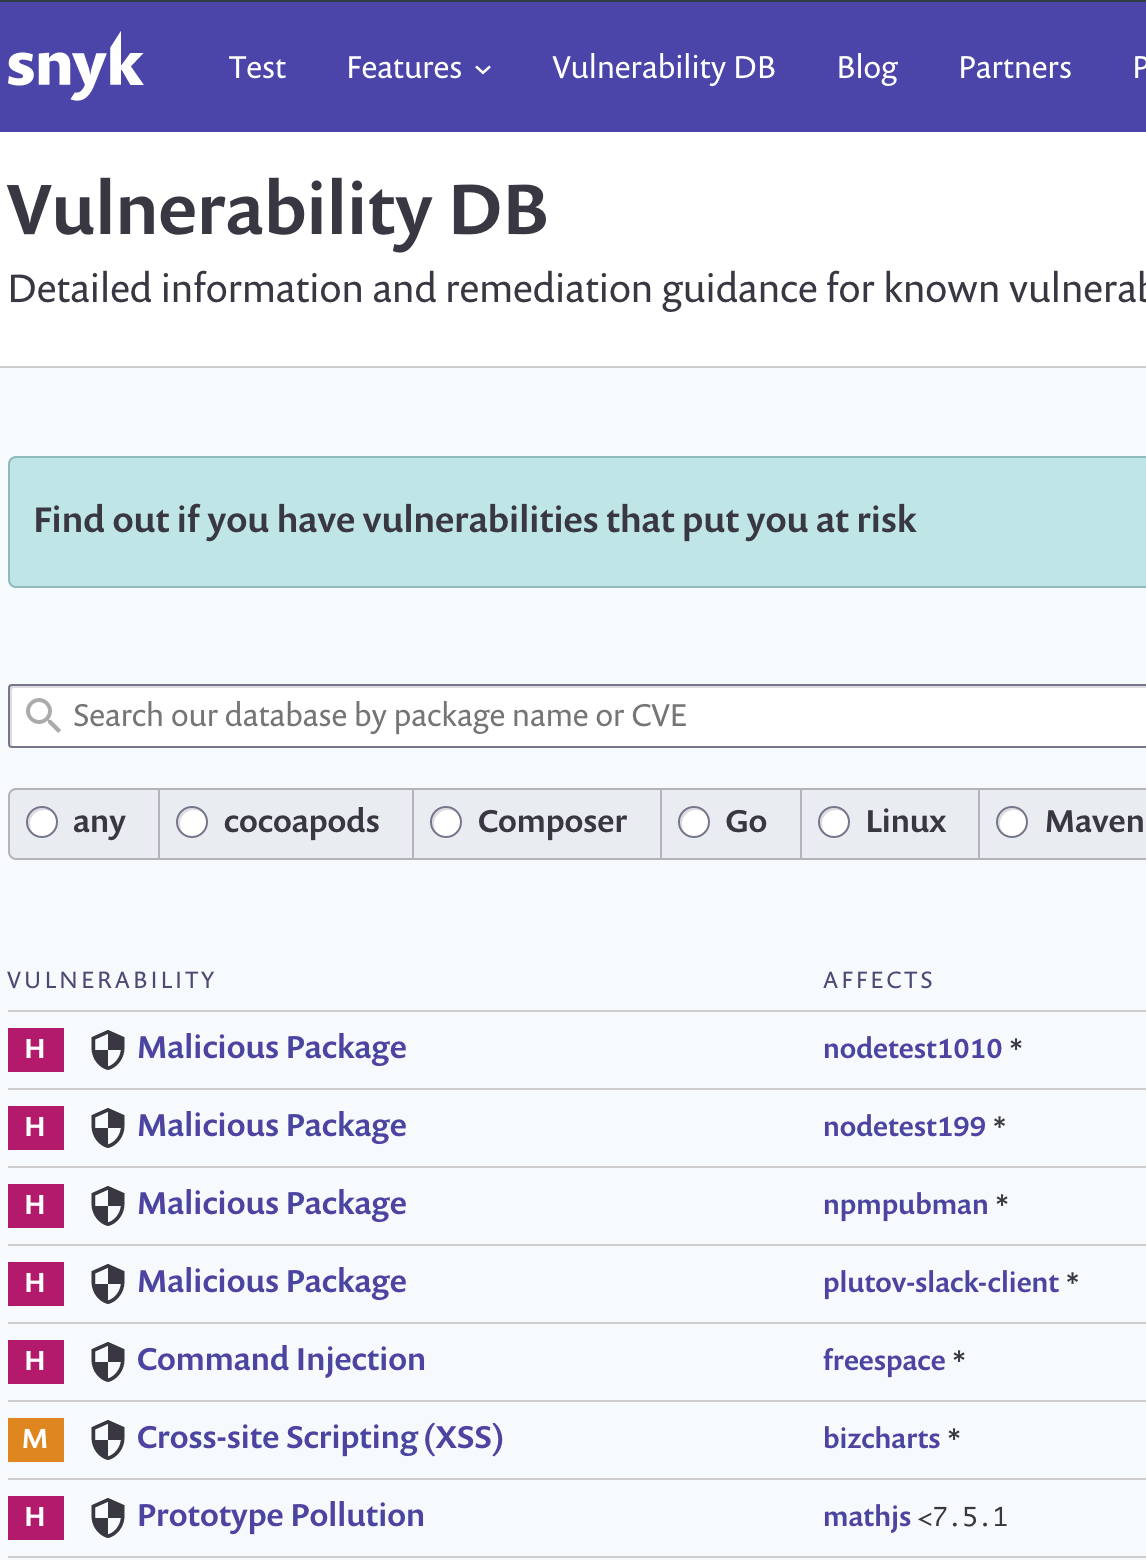
\includegraphics[width=1.4in]{figures/snyk.png}
        %\caption{fig1}
        \end{minipage}%
        }%
        \subfigure{
        \begin{minipage}[t]{0.3\linewidth}
        \centering
        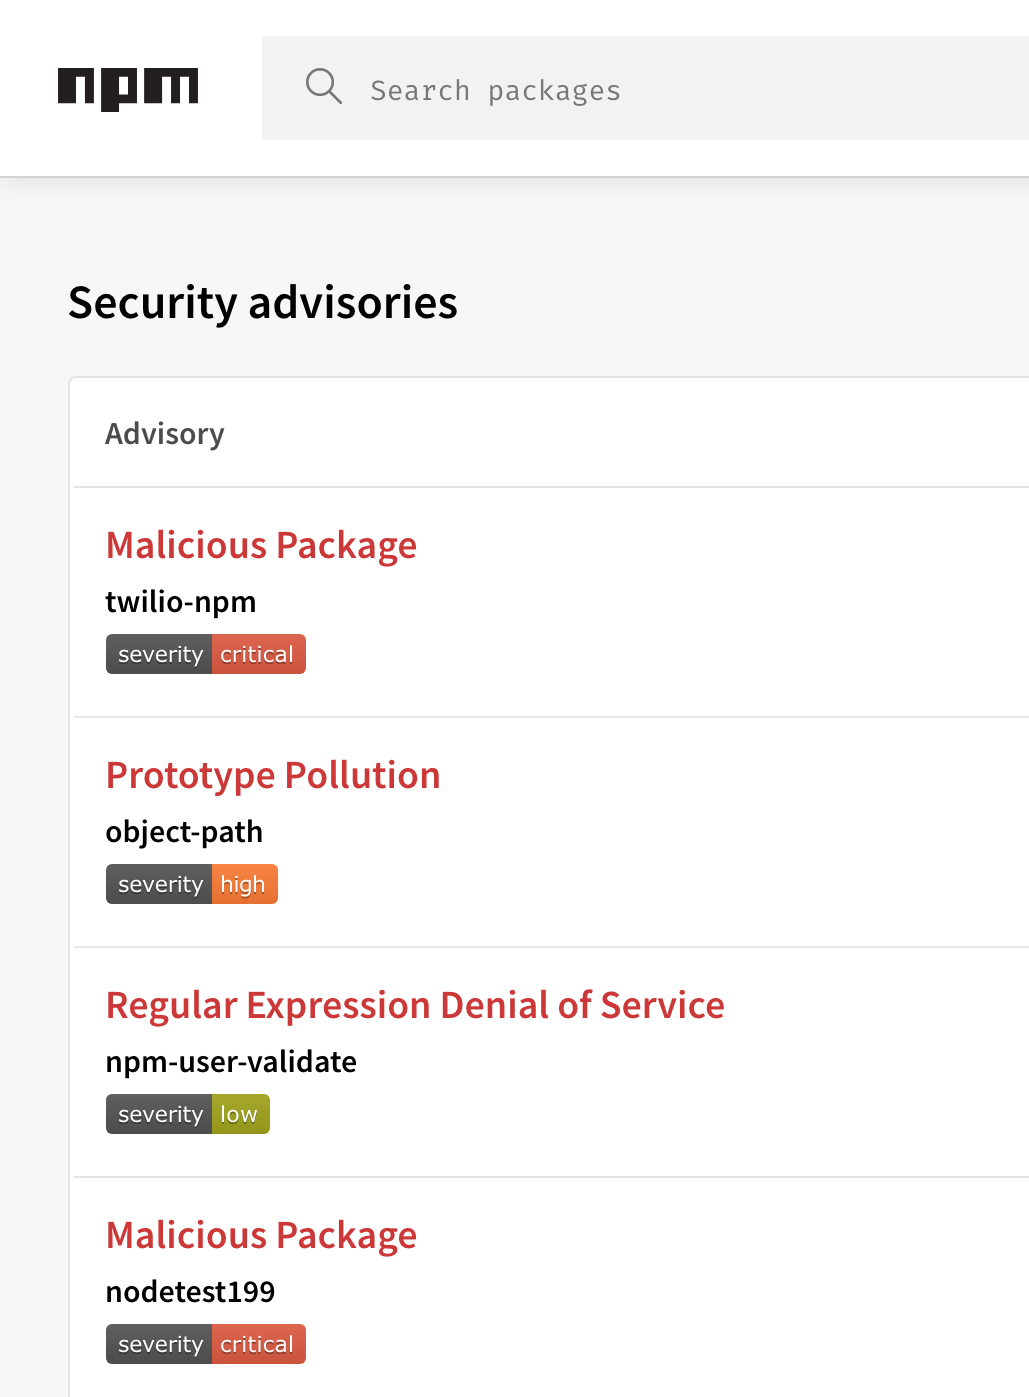
\includegraphics[width=1.4in]{figures/npm.png}
        %\caption{fig2}
        \end{minipage}%
        }%
        \subfigure{
        \begin{minipage}[t]{0.3\linewidth}
        \centering
        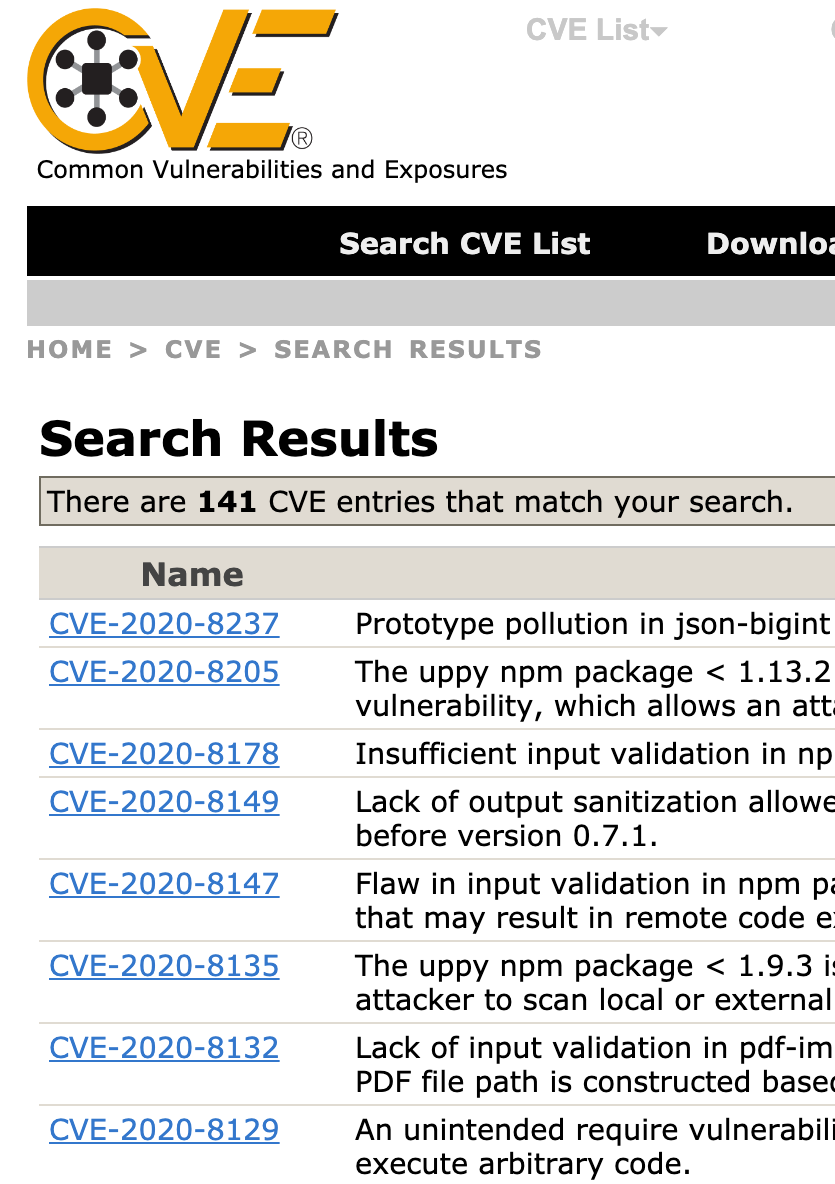
\includegraphics[width=1.4in]{figures/cve.png}
        %\caption{fig2}
        \end{minipage}
        }%
        \centering
        \caption{ Snyk.io, npm advisory and CVE.}
        \end{figure}
\end{frame}

\begin{frame}
    \frametitle{Data Source}
    NPM security advisory collects more than 1400 vulnerability reports since 2015.
    And each report provides information about the affected versions,  vulnerability overview, vulnerability detail, remediation, severity and the origin source.
    \begin{figure}[htbp]
        \centering
            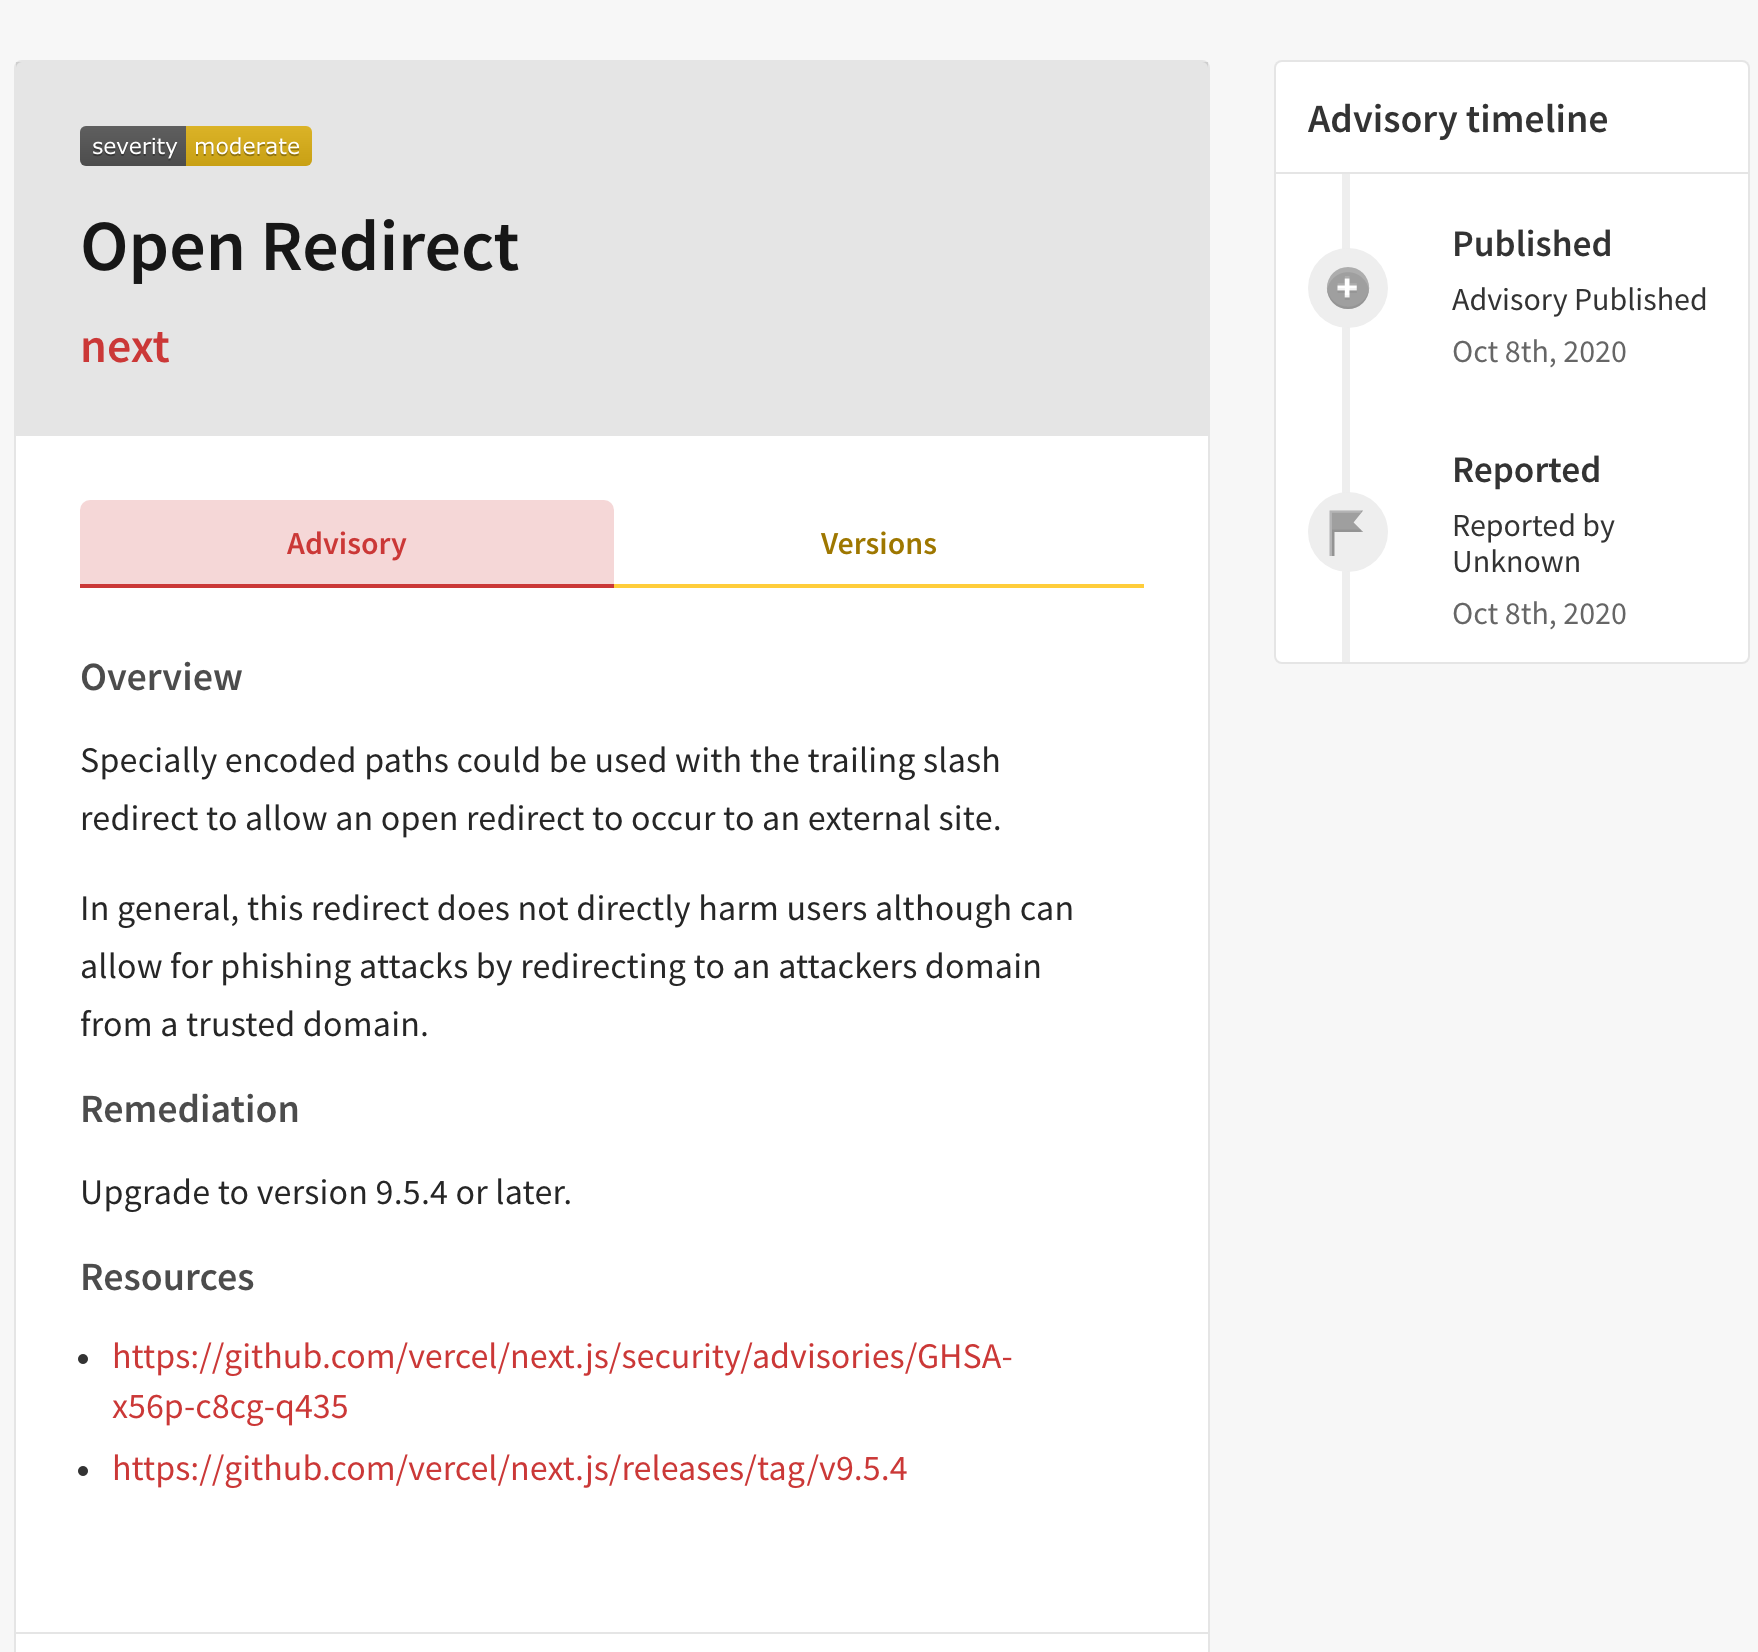
\includegraphics[width=2.0in]{./figures/advisory.png}
        \centering
        \caption{A vulnerability report example.}
    \end{figure}
\end{frame}

\begin{frame}
    \frametitle{Data Collection}
    From the npm security advisory website, we collect the vulnerability reports. The output is formatted data for easy use. 
    \begin{figure}[htbp]
        \centering
            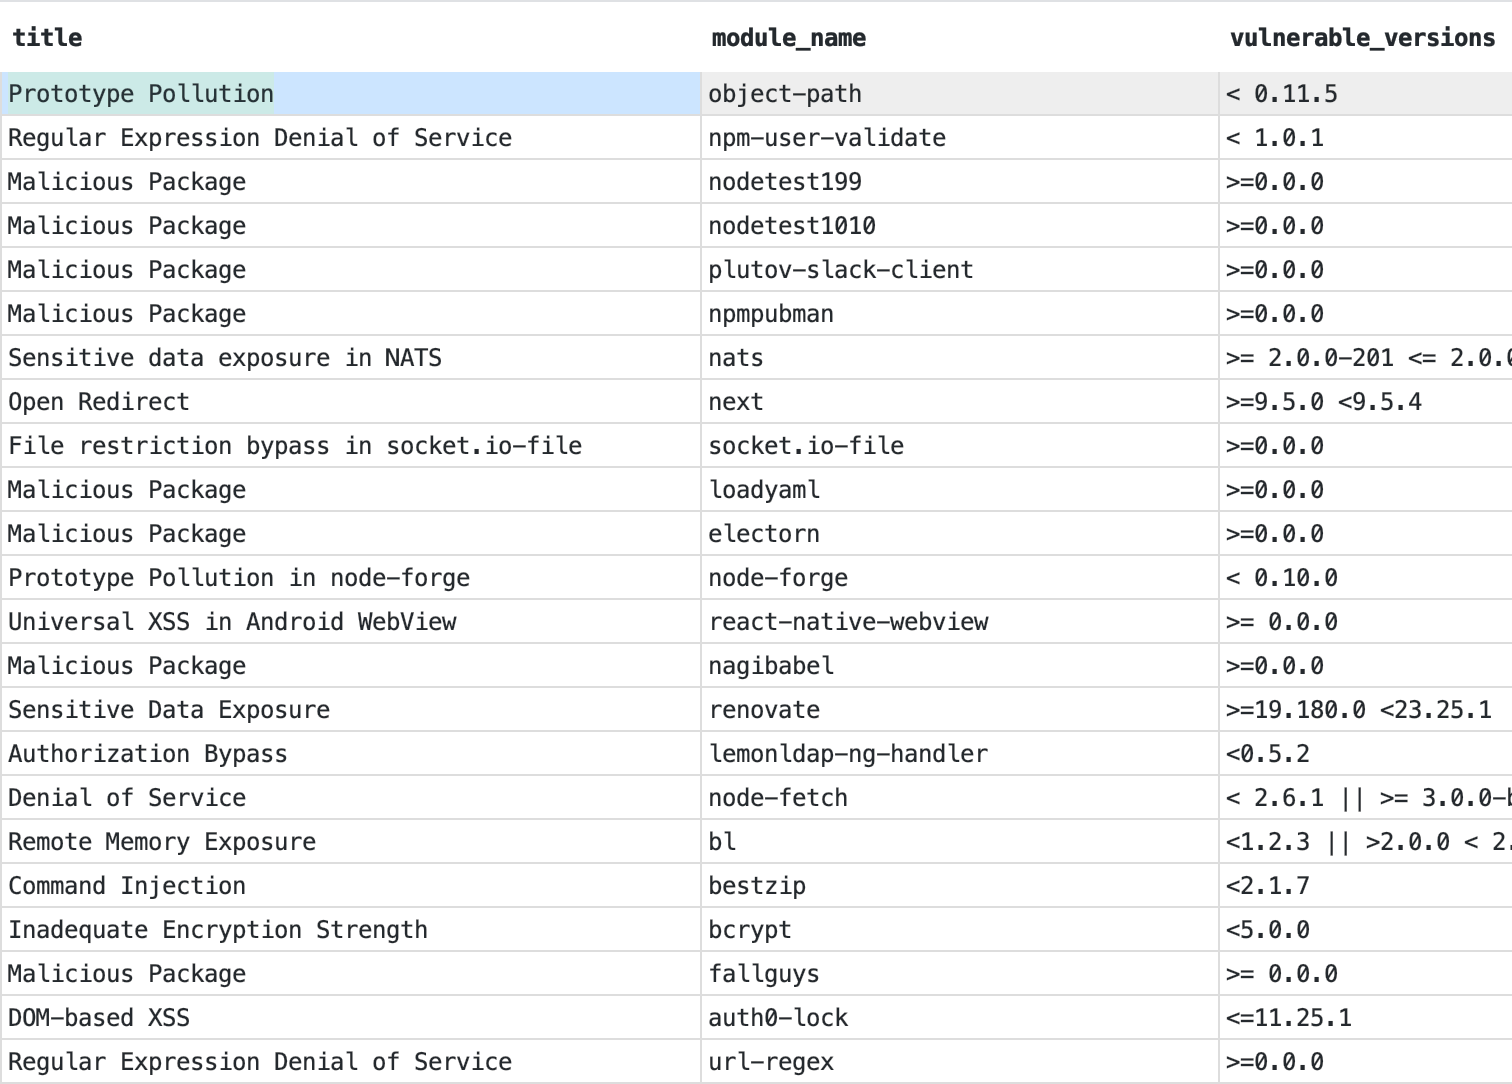
\includegraphics[width=3.0in]{./figures/sqlite.png}
        \centering
        \caption{Data collection output}
    \end{figure}
\end{frame}

\begin{frame}
    \frametitle{Severity Analysis}
    Contrary to our expectation, more than 75\% vulnerabilities are labeled as high or cirtical severity.
    \begin{figure}
        \centering
        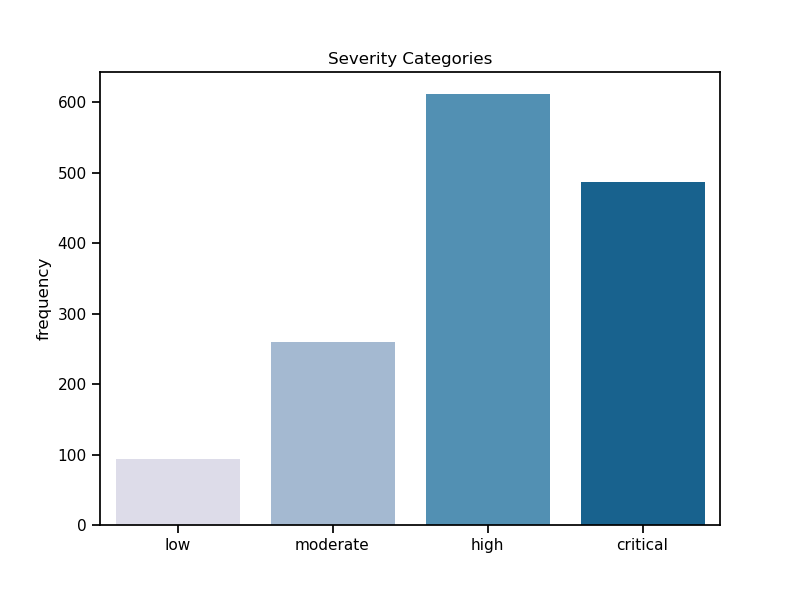
\includegraphics[width=3.3in]{./figures/severity.png}
        \centering
    \end{figure}
\end{frame}

\begin{frame}
    \frametitle{Vulnerabilities Analysis}
    We have conducted statistics on the root causes of vulnerabilities.
    \begin{figure}
        \centering
        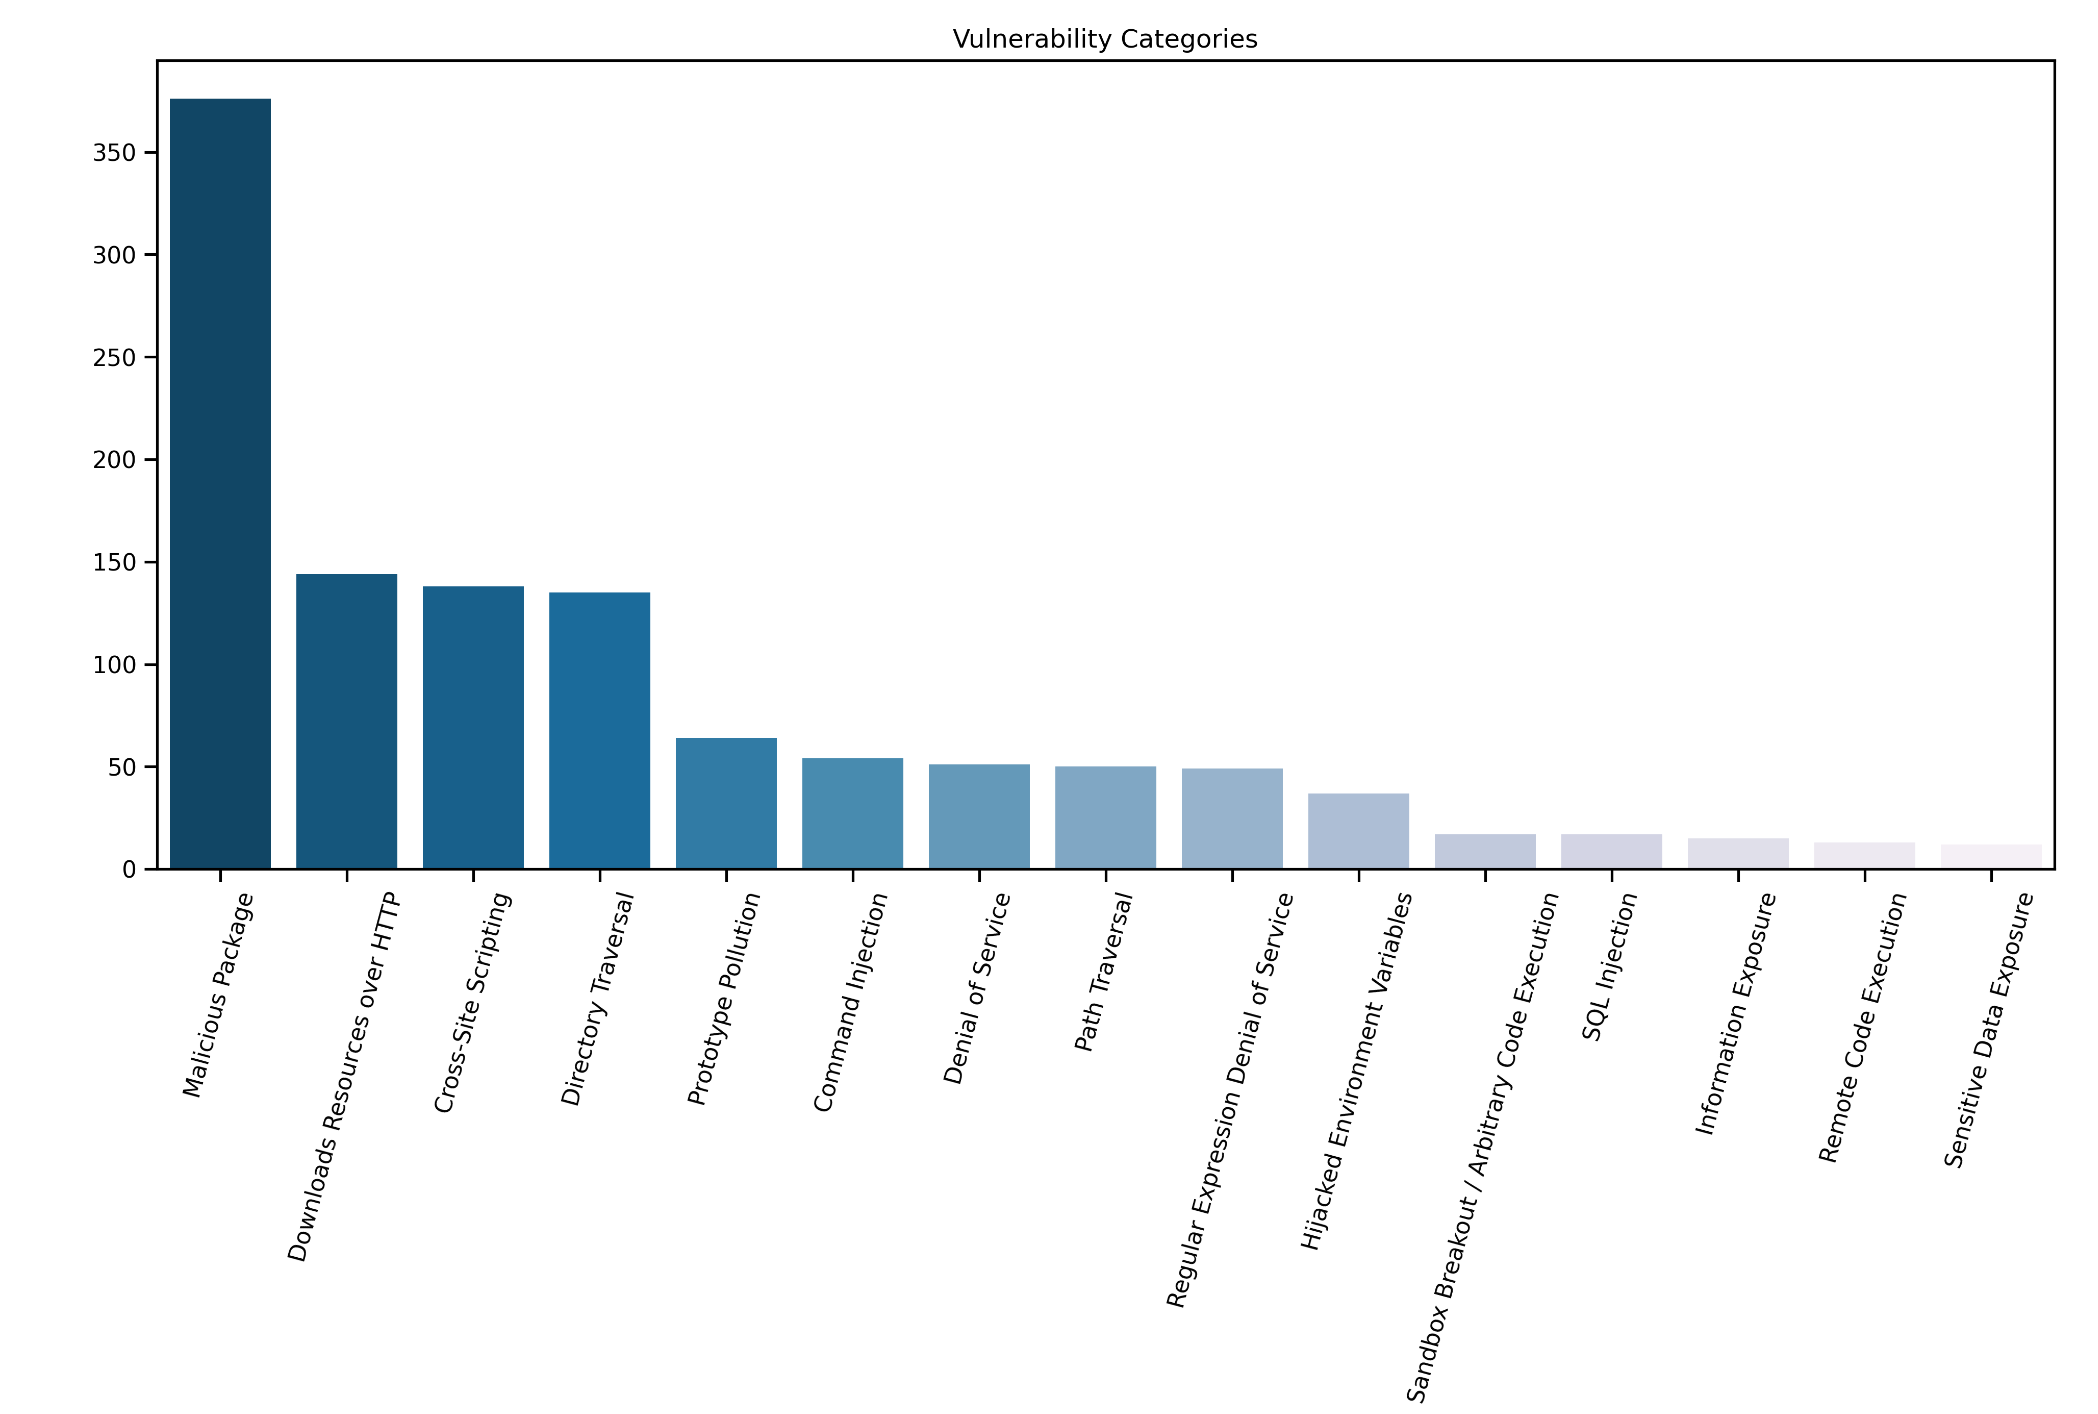
\includegraphics[width=4in]{./figures/vulnerabilities.png}
    \end{figure}
\end{frame}

\begin{frame}
    \frametitle{Typical Vulnerability Class}
    \begin{block}{Malicious Package}
        Malicious packages are packages deliberately uploaded to the npm repository by the attacker and contain malicious code. They are usually disguised as normal packages. Once reported, malicious packages will be removed from the npm repository.

        Example: 
        \begin{figure}
            \centering
            
\includegraphics[width=4in]{./figures/malicious.png}
        \end{figure}
    \end{block}

\end{frame}

\begin{frame}[fragile]
    \frametitle{Typical Vulnerability Class}
    \begin{block}{Code Injectoin}
        Code injection is the exploitation of a vulnerability that is caused by processing invalid data. Attacker use injection to introduce malicious code into a vulnerable program.

        Example:
        the package "freespace" is a library that tells user how much free disk space in a specific path. However did not check the legitimacy of the path.
    \end{block}
    \begin{lstlisting}
const freespace = require('freespace');

freespace.check('/ ; touch /tmp/semicolon_file')
.then(bytes => {
        console.log(bytes);
});
    \end{lstlisting}
\end{frame}

\begin{frame}[fragile]
    \frametitle{Typical Vulnerability Class}
    \begin{block}{Prototype Pollution}
        Prototype Pollution is about polluting the prototype of a base object which can sometimes lead to arbitrary code execution.
        
        Example: A frequently used package "lodash" which downloaded more than 30 million times a week was found to be attacked by Prototype Pollution. The function "defaultDeep" could be tricked into adding or modifying properties of "Object.prototype".
    \end{block}
    \begin{lstlisting}
const mergeFn = require('lodash').defaultsDeep;
const payload = '{"constructor": {"prototype": {"a0": true}}}'
function check() {
    mergeFn({}, JSON.parse(payload));
    if (({})[`a0`] === true) {
        console.log(`Vulnerable to Prototype Pollution via ${payload}`);
    }
  }

    \end{lstlisting}

\end{frame}


\section{Case Study}
\begin{frame}
    \tableofcontents[currentsection]
\end{frame}


\begin{frame}[fragile]
    \frametitle{Automatically Extract Dependencies}
    We developed a tool that can be used to extract a package's dependencies automatically.
    \begin{lstlisting}
        {
            "name": "ajv",
            "version": "6.6.2",
            "parent": "antd-theme-generator@1.2.8"
        },
        {
            "name": "ansi-styles",
            "version": "3.2.1",
            "parent": "antd-theme-generator@1.2.8"
        },
    \end{lstlisting}
    The output is a list that each entry of the list contains the package name, the package version and its dependent.
\end{frame}

\begin{frame}
    \frametitle{Vulnerabilities Match}
    We use this tool to build a tool chain that automatically detects potential vulnerabilities in packages.
    \begin{figure}[htbp]
        \centering
        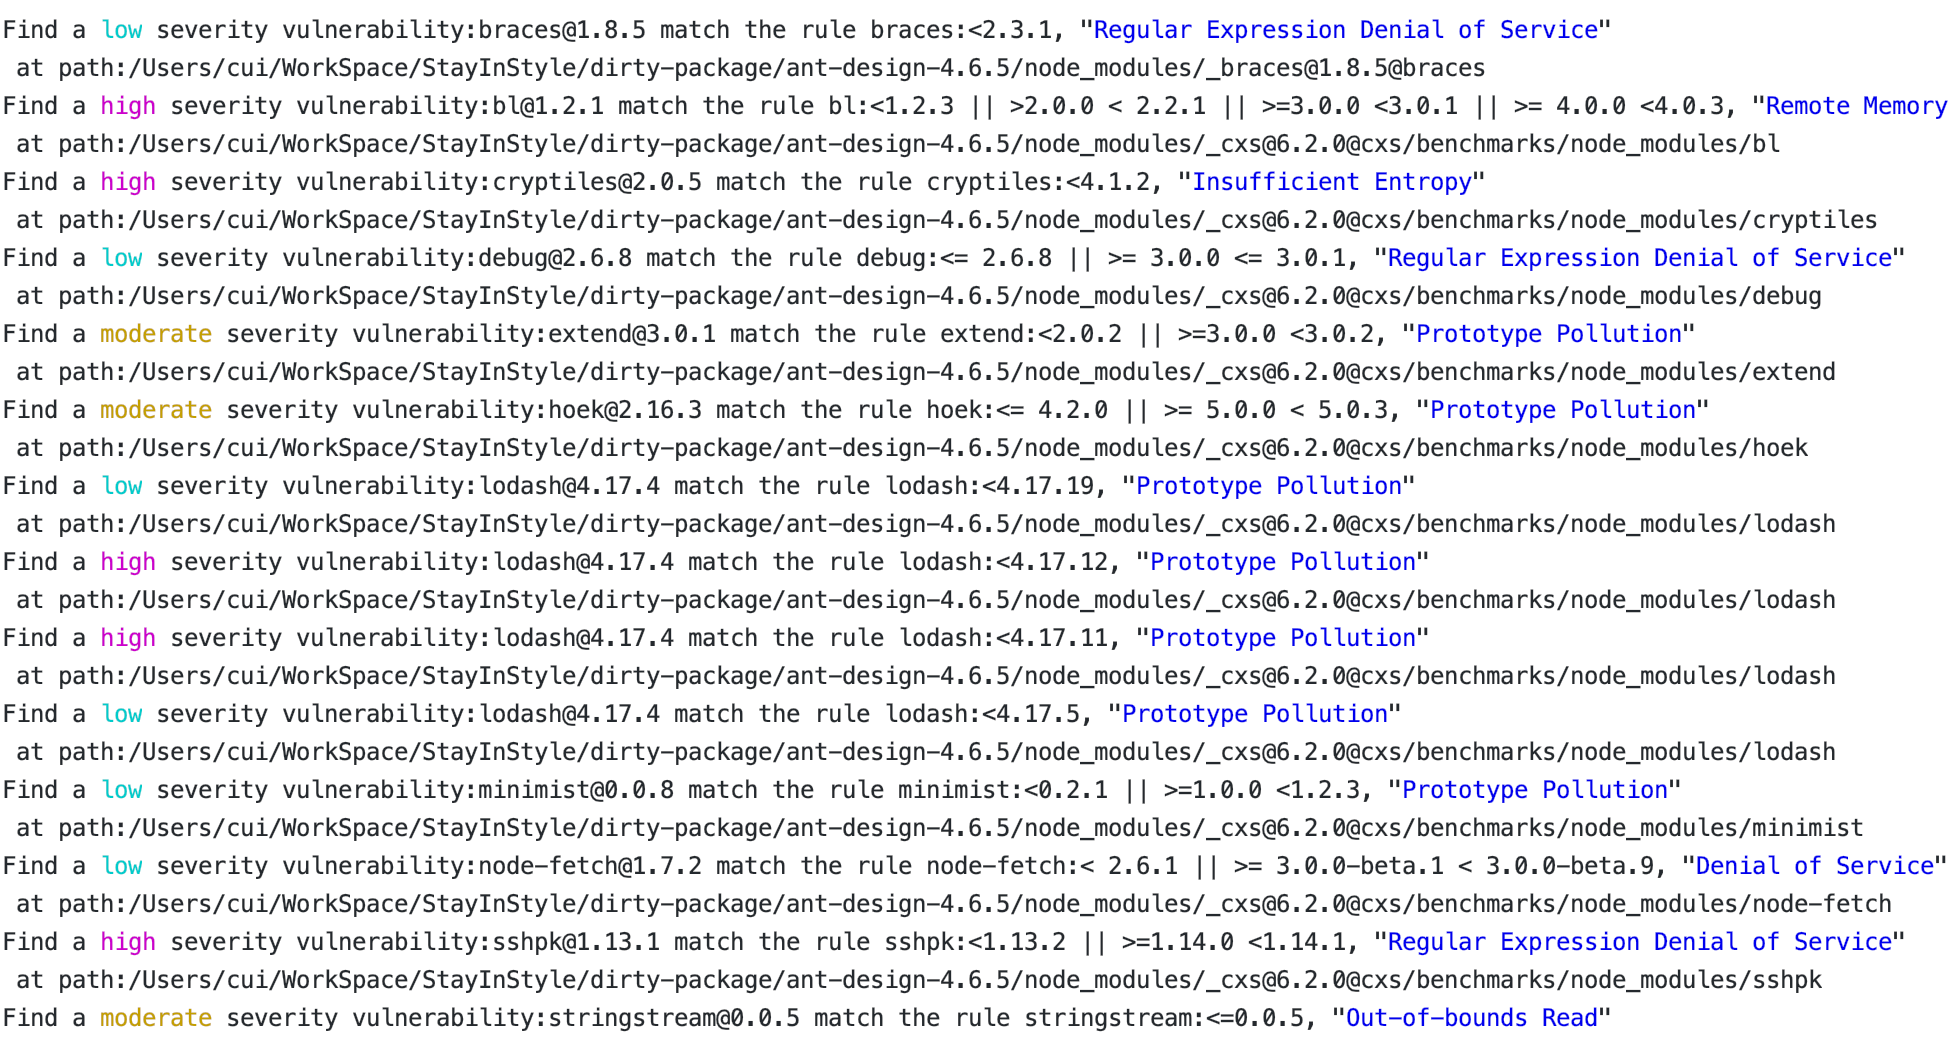
\includegraphics[width=3.5in]{figures/tool.png}
        \centering
        \caption{Partial result of detecting AntDesign package.}
    \end{figure}

\end{frame}

\begin{frame}
    \frametitle{Result}
    \centering
    %\subfloat[Decay Channels]{
     %\rule{4cm}{3cm}
     % \newcommand{\minitab}[2][l]{\begin{tabular}{#1}#2\end{tabular}}
     %\renewcommand{\multirowsetup}{\centering}
     \begin{table}
      \small   
      \begin{tabular}{|c|c|c|c|c|c|c|c|c|c|} \hline
        &antd&axios&date-fns&umi&electron&express&acorn&pm2\\
        \hline
        critical&0&1&1&0&0&0&0&0\\
        \hline
        high&6&5&1&1&0&0&0&0\\
        \hline
        moderate&4&0&2&0&0&0&0&0\\
        \hline
        low&8&8&8&3&1&3&0&0\\
        \hline
        \textbf{all}&18&14&12&3&1&3&0&0\\
        \hline
      \end{tabular}
      \centering
      \caption{Vulnerabilities in popular javascript packages.}
    \end{table}
\end{frame}

\begin{frame}
    \frametitle{Case: Axios}
    We found that the critical vulnerability in Axios is caused by "open@0.0.5".
    \begin{figure}
        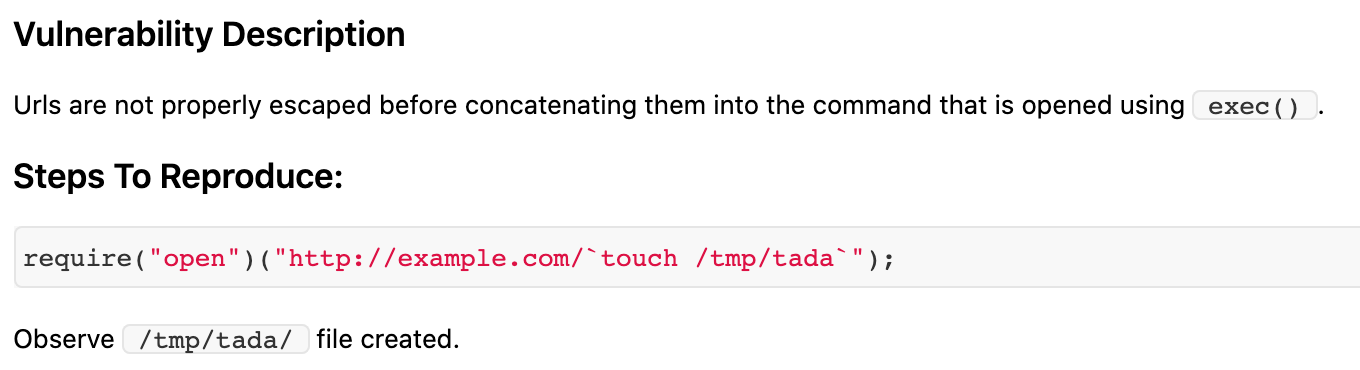
\includegraphics[width=4in]{figures/open.png}
    \end{figure}
    According to Snyk.io's vulnerability report, the older versions(<6.0.0) of "open" are vulnerable. Upgrading "open" to the last verison will prevent this vulnerability but is also likely to have unpredictable effects since it now has a very different API.
\end{frame}

\begin{frame}
    \frametitle{Case: AntDesign}
    AntDesign is a popular front-end framework. It has a complicated dependency graph. We found that if we consider its direct dependencies only, more than half of the vulnerabilities will not be detected.
    \begin{figure}
        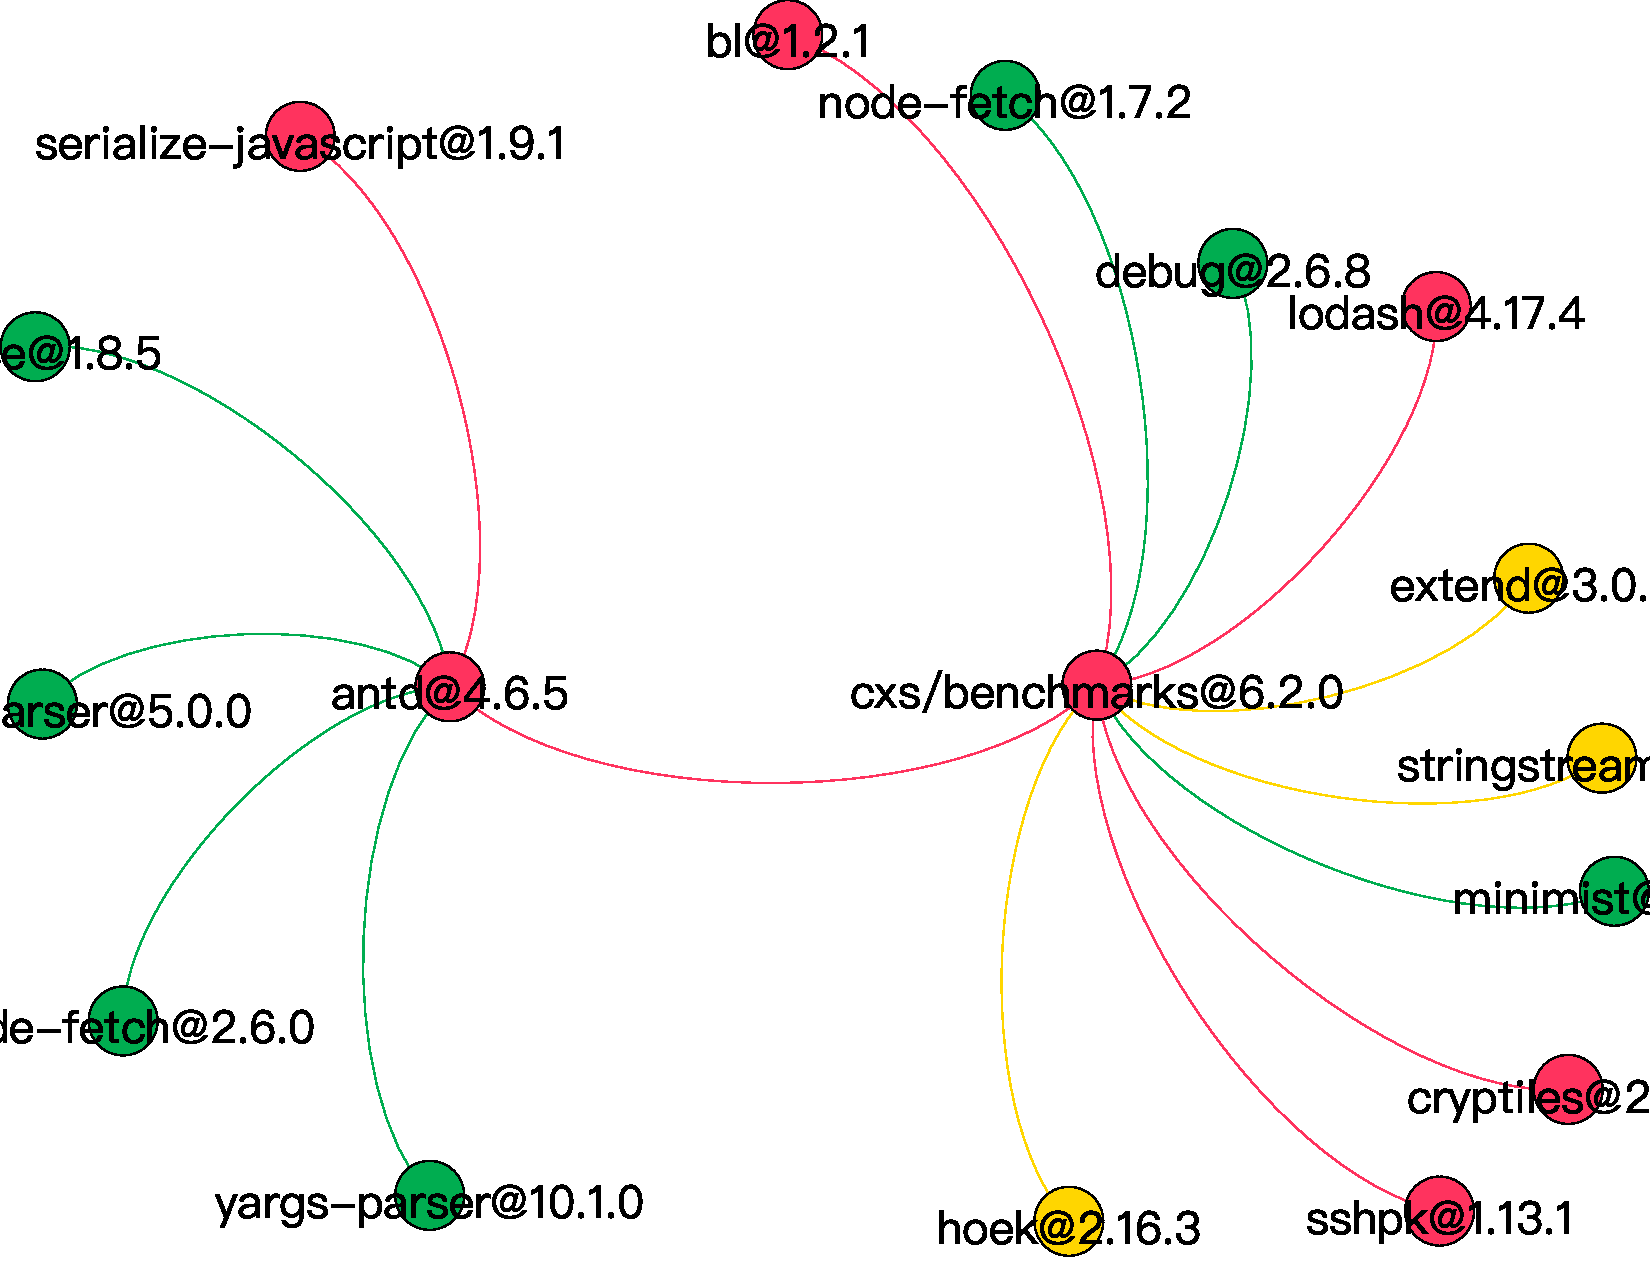
\includegraphics[width=3in]{figures/antd.pdf}
    \end{figure}
\end{frame}

\begin{frame}
    \frametitle{Study Scope}
    \begin{parchment}[Threats to Validity]
        \begin{itemize}
            \item We mainly focus on Javascript packages that use Node.js runtime.
            \item We have not analyzed on the function level yet. We mainly want to verify that the vulnerability propagation problem does exist.
            \item We select popular packages from github for analysis. These packages are mainly frameworks or function libraries. We do not analyze applications.
        \end{itemize}
    \end{parchment}
\end{frame}


\section{Summary \& Future Work}
\begin{frame}
    \tableofcontents[currentsection]
\end{frame}

\begin{frame}
    \frametitle{Summary}
    \begin{block}{Work Summary}
    \begin{itemize}
        \item We built a tool chain that automatically detects vulnerabilities in npm packages.
        \item We analyzed some popular npm packages.
    \end{itemize}
    \end{block}

    \begin{block}{Preliminary Conclusion}
            We found high-risk vulnerabilites in some of the popular packages we detected which is concrete evidence to support the existence of this problem.
    \end{block}
\end{frame}

\begin{frame}
    \frametitle{Future Work}
    \begin{parchment}[How to get down to the function level?]
    \textbf{A Naive Idea Using Approximate Analysis}: 

    Because the lack of basic functions in JavaScript's standard library, there are numerous micro-packages with very few lines of code in npm repository[1]. These small-scale packages contain few functions. Thus if we find a package is vulnerable, we simply mark all of its functions as vulnerable.
    \begin{itemize}
        \item Good news: no false-negative;
        \item Bad news: not precise enough;
    \end{itemize}
        
    \end{parchment}
    \footnote{Markus Zimmermann, Cristian-Alexandru Staicu, Cam Tenny, \& Michael Pradel (2019). Small World with High Risks: A Study of Security Threats in the npm Ecosystem. In 28th USENIX Security Symposium (USENIX Security 19) (pp. 995–1010). USENIX Association.}
\end{frame}

\begin{frame}
    \frametitle{Future Work}
    \begin{parchment}[How to get down to the function level?]
    \textbf{Mining Text Information:}

    In the process of data collection, we find that some of the vulnerabilites reports mentioned the specifics vulnerable functions at the vulnerability overview. 
    \begin{itemize}
        \item Good news: According to our research, quite a few vulnerabilities report have related overview pointing out the location of the vulnerability.
        \item Bad news: How to acquire the information we need from raw text? 
    \end{itemize}
    
    \end{parchment}
    \begin{figure}
        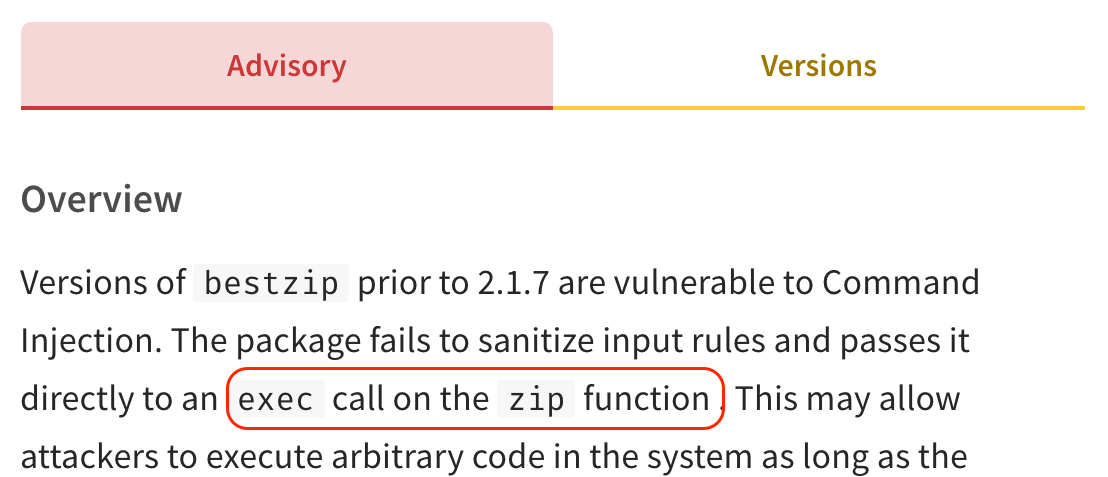
\includegraphics[width=2in]{figures/function.png}
    \end{figure}

\end{frame}

\begin{frame}
    \frametitle{Future Work}
    \begin{parchment}[How to get down to the function level?]
    \textbf{Comparing Different Versions:}

    Since we already know the vulnerable versions, we can compare the last vulnerable verison package and the first patched version package and the unchanged functions is clear.

    Bad news: 
    \begin{itemize}
        \item Can not rule out some performance optimization changes.
        \item What if there is no patched version?
    \end{itemize}
    \end{parchment}
\end{frame}

\begin{frame}
    \centering \Large
    \emph{\textcolor{AmethystPurple}{Thanks. Q\&A}}
\end{frame}

\end{document}